\documentclass[10pt,a4paper]{article}
\usepackage[ngerman,english]{babel}
\usepackage[utf8]{inputenc}
\usepackage{hyperref}
\usepackage{graphicx}
\usepackage{algpseudocode}
\usepackage{amssymb}
\usepackage{amsmath}
\usepackage{listings}
\title{Polytopes}
\author{Henrique Hepp}
\newcommand{\Tau}{\mathcal{T}} 
\begin{document}
\maketitle

Algorithm based on the article ``Embedding Stacked Polytopes on a Polynomial-Size Grid''.

The algorithm can be divided in:

\begin{enumerate}
\item Receive the entry.
\item Heavy caterpillar decomposition.
\item Balance the tree.
\item Get the coefficients.
\item Lift the graph to a polytope. 
\end{enumerate}


\section{The Entry of the algorithm}

It is given to the algorithm a 3 connected planar graph and a tree representation of the graph, as showed below.

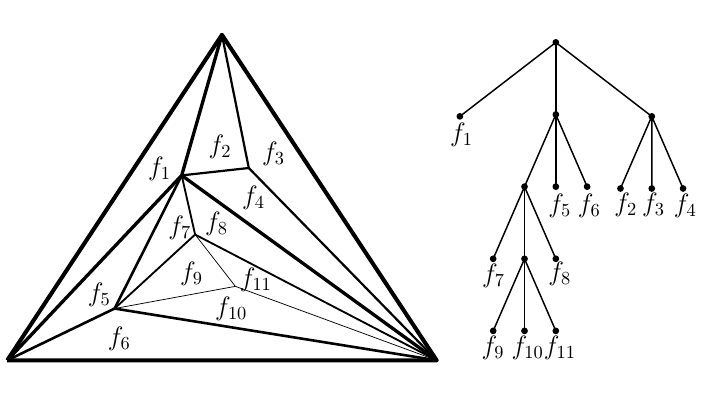
\includegraphics[scale=0.8]{graph_tree.png} 

\section{Heavy caterpillar decomposition}
The tree representation is decomposed in \textit{heavy paths}. Resulting sub-trees called \textit{caterpillars}. When a node lies on a heavy path it is called a \textit{spine node}, otherwise is a \textit{tree node}. The spine nodes are labelled by $s_1$ (root), $s_2$, ..., $s_i$,...,$s_\bot$. The children from $s_i$ are $s_{i+1}$, $t_{i+1}$ and $t'_{i+1}$. In $t$ are stored a pointer link$(t)$ to a other caterpillar. 

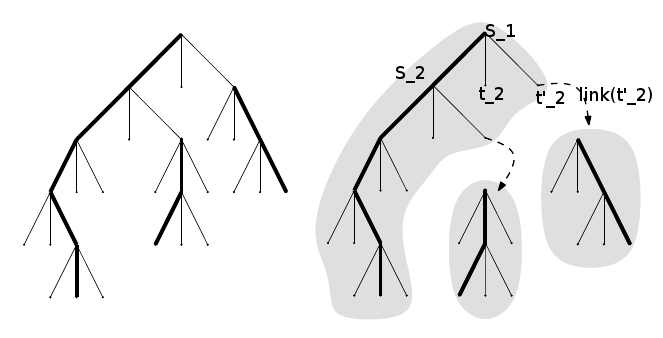
\includegraphics[scale=1]{caterpillarEdit.png} 

\section{Balance the tree}
\begin{algorithmic}
\Function{BALANCE}{C} 
\State \textbf{Input:} A caterpillar $C$ from the heavy caterpillar decomposition of $\Tau(G)$. All weights are equal 1.
\State \textbf{Output:} Weights for the nodes of $\Tau(G)$.

\ForAll{$t_i$, $t'_i$ in $C$} 
	\State BALANCE(link($t_i$))
	\State BALANCE(link($t'_i$))
    \If {$w(t_i)>w(t'_i)$}
        \State relabel $t_i \leftrightarrow t'_i$
    \EndIf
	\State $w(t_i)=w(t'_i)$
	\State add $(w(t_i ) - w(t'_i ))$ to the weight of $s_{\bot}$ in link $(t_i)$
	\State add $(w(t'_i ) - w(t_i ))$ to the weight of link$^{-1} (C)$
\EndFor
\EndFunction
\end{algorithmic}


A balanced Tree:

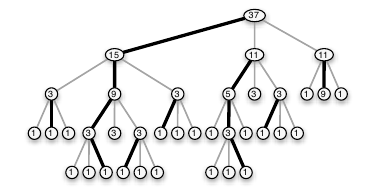
\includegraphics[scale=1]{balancedTree.png} 


\section{Get the coefficients}

If $v_i$ is the vertex stacked on the face $v_jv_kv_l$ then:

$$\alpha_{ijkl} = \frac{1}{w(t_u)}$$

Where $w(t_u)$ is the weight of the subface $v_jv_kv_l$ obtained by the function BALANCE.

The weights are now updated with the coordinate values. First the coordinates from the vertices are rounded down. $r_i = (\lfloor x_i \rfloor, \lfloor y_i\rfloor)$.

The weights are:

$$\dot{w}_{ij}= \sum_{\{i,j,k,l\}\in S} \lfloor Y \alpha_{ijkl}\rfloor w^{kl}_{ij}$$   

The coefficient $\alpha_{ijkl}$ is scaled by multiplying it with $Y = 4 n^2$, $n$ is the number of vertices.


$$w^{kl}_{ij}= [i,k,l][j,k,l]$$

$$
[i,j,k]= \text{det}
 \begin{pmatrix}
  x_i & x_j & x_k\\
  y_i & y_j & y_k\\
  1	  & 1   & 1  \\
 \end{pmatrix}
$$

\section{The lifting}

Pages 133 to 139 of REALIZATION SPACES OF POLYTOPES



\end{document}
